\chapter{Specific Requirements}
\section{Scenarios}
\subsection{Registration to the service}
\subsubsection{Scenario}
Bob has discovered the new service offered by the city called \textit{myTaxiService} and he wants to discover how it works. He goes to the web application site and starts the registration phase.\\
He insert a the username and the password he wants and submit the request of registration. The system replies saying that the username selected is already used and that Bob has to insert another username. Bob insert another username and this time the procedure succeed. Bob is now correctly registered to \textit{myTaxiService}.

\subsubsection{Use case}
\begin{center}
\centering
\begin{longtable}{| p{.20\textwidth} | p{.80\textwidth} |} \hline
Use case & \textbf{Register} \\ \hline 
Actors & Passenger \\ \hline
Goals & A passenger must be able to register to the service \\ \hline
Enter condition & None \\ \hline
Event flow & \begin{enumerate}
				\item The passenger goes to the web application page
				\item The passenger clicks on the sign up button
				\item \label{fillForm1} The passenger fills the form with username and password desired
				\item The passenger clicks the submit button
				\item If the username is already present in the system or there are missing data
				\begin{enumerate}
					\item Notify the Passenger of the error
					\item Go back to Event flow \ref{fillForm1}
				\end{enumerate}	
				\item The system retrieves the data and stores them
				\item The system notifies that the registration has been correctly done
			\end{enumerate} \\ \hline
Exceptions & If the user, during the insertion of the registration data (username + password) decides to abort the procedure by clicking on the proper button
			\begin{enumerate}
				\item The system notifies the passenger of the loss of the inserted data
				\item The system abort the procedure
			\end{enumerate}\\ \hline
Exit condition & The passenger is correctly registered to the service \\ \hline
\caption{Use case: Register}
\end{longtable}
\end{center}

\pagebreak
\subsection{Passenger Reservation}
\subsubsection{Scenario}
It is 9.00 in the morning and Tom has already downloaded the mobile application called \textit{myTaxiService} and he has a fixed appointment at 17.00 at "Stazione Centrale of Milano" so he decides to reserve a taxi for the 16.30 to go there. He enters in the apposite section of the application, indicates the source of the journey,the destination, the time of the meeting with the Taxi driver. He also specify the number of passengers that the Taxi will carry. The system, after a few seconds, reply positively to Tom saying that the reservation has been accepted and that the Taxi identification number will be provided 10 minutes before the meeting time.

\subsubsection{Use case}
\begin{center}
	\begin{longtable}{| p{.20\textwidth} | p{.80\textwidth} |} \hline
		Use case & \textbf{Reserve a taxi} \\ \hline 
		Actors & Passenger, Taxi Driver \\ \hline
		Goals & A passenger must be able to reserve a taxi ride from an origin, to a destination at a specific time and date \\ \hline
		Enter condition & \begin{itemize}
			\item The Passenger must already be registered to the service
			\item The Taxi driver must be registered to the service
			\item The Passenger must already have opened the application (mobile or web) and logged in
			\item The Taxi driver must be available to accept requests
		\end{itemize} \\ \hline
		Event flow & \begin{enumerate}
			\item The Passenger goes to the section for reserving a taxi ride
			\item \label{fillForm} The Passenger fills the form with: origin, location, date, time, number of passengers			
			\item The Passenger submit the request to the system
			\item If there are errors with the data (missing fields, not valid locations or number of passengers greater than 3) or the date and time provided are not 2 hours in advance:
			\begin{enumerate}
				\item The system notifies the error to the Passenger
				\item Go back to Event flow \ref{fillForm}
			\end{enumerate}
			\item The reservation is stored in the system
			\item The system waits until 10 minutes before the date and time of the reservation
			\item The system checks the origin location provided by the Passenger and computes the corresponding zone in the city
			\item The system, based on the city zone computed, retrieves the corresponding taxi queue
			\item If there are no taxi in the queue: \label{noTaxi}
			\begin{enumerate}
				\item Returns an error to the Passenger and invites him to make a request
				\item Go back to Event flow \ref{fillForm}
			\end{enumerate}
			\item The system takes the first taxi in the queue
			\item The system send the request to the taxi driver
			\item If the taxi driver does not accept the request:
			\begin{enumerate}
				\item The system puts the Taxi driver at the bottom of the queue
				\item Go back to Event flow \ref{noTaxi}
			\end{enumerate}
			\item The system sends to the Taxi driver the location of the meeting point with the Passenger
			\item The system computes an approximate waiting time for the Passenger
			\item The system informs the Passenger of the forthcoming arrival of the Taxi and the approximate waiting time.
		\end{enumerate} \\ \hline
		Exceptions & The passenger can abort the procedure only during the	waiting phase. If he decides to abort the procedure:
		\begin{enumerate}
		\item If the time of cancellation of the reservation is later than 10 minutes before the meeting time:
		\begin{enumerate}
			\item The system notifies the Passenger of the impossibility to cancel the reservation
		\end{enumerate}
		\item The system cancel the reservation
		\item The system notifies the Passenger of the successful deleting of the reservation
		\end{enumerate} \\ \hline
Exit condition & The passenger is waiting for the taxi driver and a Taxi driver is reaching him
		\\ \hline
		\caption{Use case: Taxi reservation from a passenger}+
		\label{reserveTaxiUC}
	\end{longtable}
\end{center}

\subsubsection{Sequence diagram}
\begin{figure}[H]
\centering
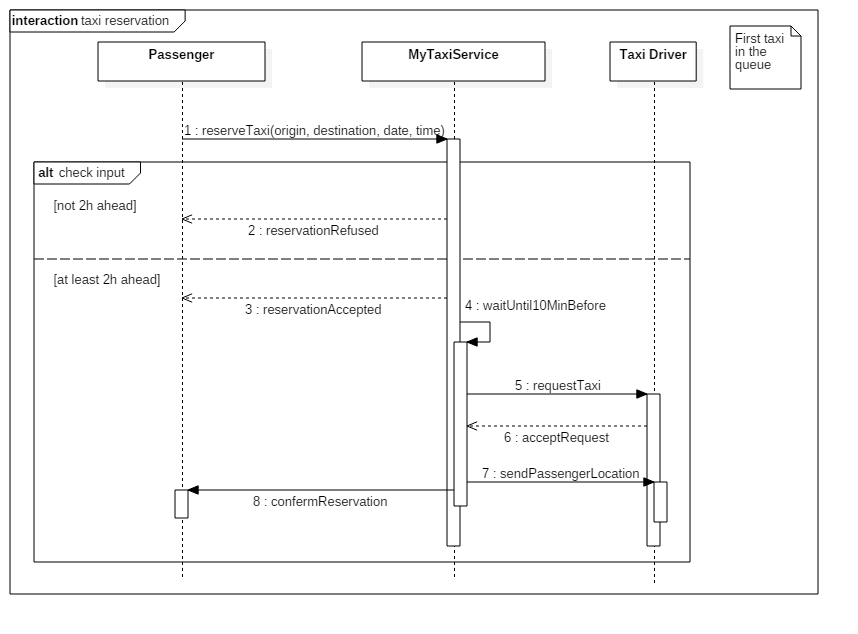
\includegraphics[scale=0.5]{Images/sequence_taxi_reservation}
\caption{Reservation of a taxi}
\label{reserve_taxi_SD}
\end{figure}




\subsection{Passenger immediate request}
\subsubsection{Positive response}
Tom has already download the mobile application called \textit{myTaxiService} and desire to request a taxi ride from his actual place, located in "Piazzale Gorini 18, Milano" to the "Stazione Centrale of Milano". He enters in the immediate request section of its application, fills the form (source of the journey, number of passengers) and waits for a response from the service.
After a few seconds the system responds indicating that the taxi with identification code T345 is arriving at the requested address. The approximate waiting time for the taxi is 5 minutes.

\begin{figure}[H]
\centering
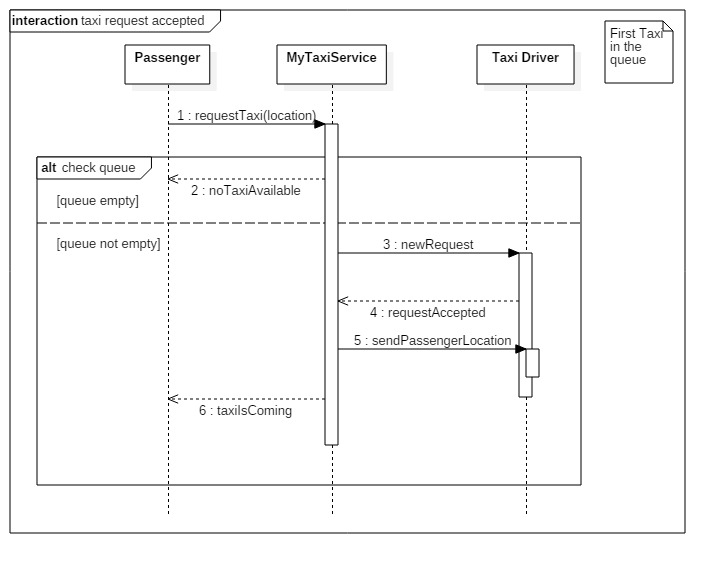
\includegraphics[scale=0.6]{Images/sequence_taxi_request_accepted}
\end{figure}

\subsubsection{Use case}
\begin{table}[H]
\centering
\begin{longtable}{| p{.20\textwidth} | p{.80\textwidth} |} \hline
Use case & \textbf{Request a taxi} \\ \hline 
Actors & Passenger, Taxi Driver \\ \hline
Goals & A passenger must be able to register to the service \\ \hline
Enter condition & \begin{itemize}
					\item The Passenger must already been registered to the service
					\item The Taxi driver must be registered to the service
					\item The Passenger must already have opened the application (mobile or web) and logged in
					\item The Taxi driver must be available to accept requests
					\end{itemize} \\ \hline
Event flow & \begin{enumerate}
				\item The Passenger goes to the section for requesting an immediate taxi
				\item \label{fillForm} The Passenger fills the form with:
				\begin{itemize}
					\item Meeting location
					\item Number of passengers
				\end{itemize}
				\item The Passenger submit the request to the system
				\item If there are missing data or the specified location is not valid or the number of passengers is greater than 3:
				\begin{enumerate}
					\item The system notifies the error to the Passenger
					\item Go back to Event flow \ref{fillForm}
				\end{enumerate}
				\item The request is stored in the system
				\item The system checks the location provided by the Passenger and computes the corresponding zone in the city
				\item The system, on the base of the city zone computed, retrieves the corresponding taxi queue
				\item If there are no taxi in the queue:
				\begin{enumerate}
					\item Returns an error to the Passenger and invites him to retry later
					\item Go back to Event flow \ref{fillForm}
				\end{enumerate}
				\item The system takes the first taxi in the queue
				\item The system send the request to the taxi driver
				\item If the taxi driver does not accept the request:
				\begin{enumerate}
					\item AD
				\end{enumerate}
			\end{enumerate} \\ \hline
\end{longtable}
\caption{Use case: Taxi request from a Passenger}
\end{table}


\subsubsection{Negative response}
Tom has already download the mobile application called \textit{myTaxiService} and desire to request a taxi ride from his actual place, located in "Piazzale Gorini 18, Milano" to the "Stazione Centrale of Milano". He enters in the immediate request section of its application, fills the form (source of the journey, number of passengers) and waits for a response from the service.
After a minute the system responds indicating that there are no taxi available in the corresponding zone and Tom is invited to retry later.
\begin{figure}[H]
\centering
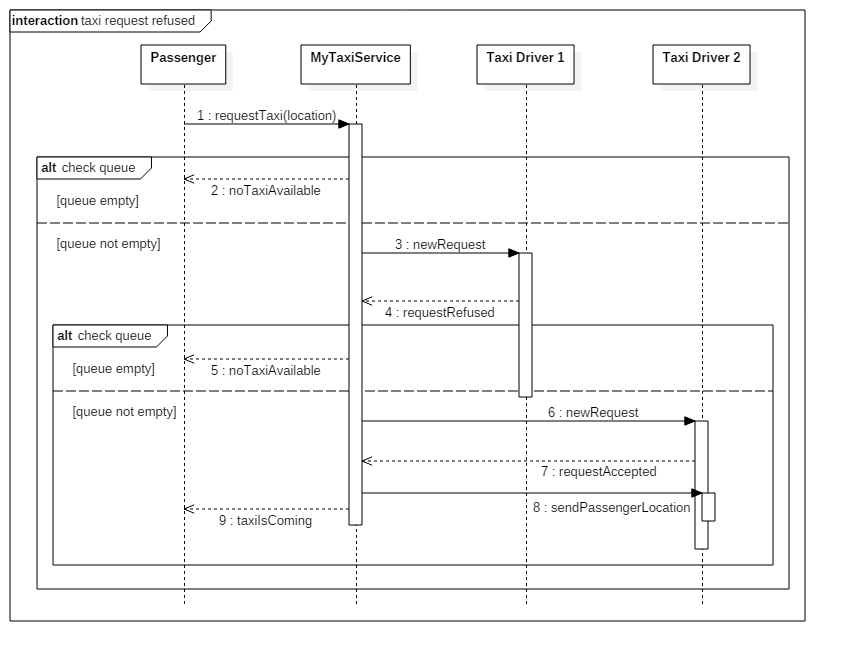
\includegraphics[scale=0.5]{Images/sequence_taxi_request_refused}
\end{figure}

\subsubsection{Functional requirements}

\pagebreak
\subsection{Taxi driver: start of the working day}
\subsubsection{Scenario}
Bob is a Taxi driver that works in the large city and has already installed the application \textit{myTaxiService - Taxi Driver Edition}.
He enter in his taxi and opens the mobile application. In the home page of the application he press the button which himself as available. The system automatically stores the identifier of his taxi in the queue corresponding at the location of the taxi (given by the GPS system of his smart phone).
A message of the system says to Bob that his taxi has been inserted in a waiting queue and a waiting screen appears.

\subsubsection{Use case}
\begin{center}
\begin{longtable}{| p{.20\textwidth} | p{.80\textwidth} |} \hline
	Use case & \textbf{Start working} \\ \hline 
	Actors & Taxi Driver \\ \hline
	Goals & A Taxi Driver must be able to set himself as available (start working)  \\ \hline
	Enter condition & \begin{itemize}
						\item The Taxi Driver must be already registered to the service
						\item The Taxi Driver must already have opened the application
						\end{itemize} \\ \hline
	Event flow & \begin{enumerate}
					\item The Taxi Driver press on the apposite button with the intention of setting himself as available
					\item The system receives the updated status of the Taxi Driver
					\item The system retrieves the location of the Taxi Driver from the GPS system
					\item The system computes the actual zone of the Taxi Driver
					\item The system puts the taxi driver at the bottom of the taxi queue relative to the computed taxi zone.
					\item The system notifies the Taxi Driver and now he is waiting for a request
				\end{enumerate} \\ \hline
	Exit condition & The Taxi Driver is waiting in a Taxi Queue\\ \hline
	\caption{Use case: Taxi Driver starts working}
\end{longtable}
\end{center}
\subsection{Taxi driver: acceptance of a request}
Bob is a Taxi driver that works in the large city and has already installed the application \textit{myTaxiService - Taxi Driver Edition}.
He is in the middle of his working day (so he has already executed the procedure at "Taxi driver: start of the working day") and he is waiting in a taxi queue corresponding to his actual location in the city.\\
Suddenly a pop-up shows up saying that there is a new request for a ride and he is asked to say if he wants to accept it or not.
He press the button "YES" and another screen opens specifying the location of the Passenger. The systems automatically sets the Bob's taxi as "busy" (not available): the taxi is removed from the taxi queue\\
Bob go to the location specified, picks up Alice and brings her to her desired location. At the end of the ride, Bob press the button "End of the ride" on the screen. The system computes his actual location and puts him in the nearest taxi queue.

\subsubsection{Use case}
See table \ref{requestTaxiUC} and table \ref{reserveTaxiUC}.

\subsubsection{Sequence diagram}
See figure \ref{request_positive_TaxiSD}, \ref{request_negative_TaxiSD} and \ref{reserve_taxi_SD}
\subsection{Taxi driver: refusing a request}
Bob is a Taxi driver that works in the large city and has already installed the application \textit{myTaxiService - Taxi Driver Edition}.
He is in the middle of his working day (so he has already executed the procedure at "Taxi driver: start of the working day") and he is waiting in a taxi queue corresponding to his actual location in the city.\\
Suddenly a pop-up shows up saying that there is a new request for a ride and he is asked to say if he wants to accept it or not.\\
He press "NO" because he \textit{wants to watch the world burn} (Batman citation)

\subsubsection{Use case}
See table \ref{requestTaxiUC} and table \ref{reserveTaxiUC}
\subsection{Taxi driver: end of working day}
\subsubsection{Scenario}
Bob is a Taxi driver that is finishing his working day. He has just finished his last ride and the passenger has just left the taxi. He takes his phone with the application \textit{myTaxiService} already running. He communicates to the system that he has ended the current ride. The system puts him in the taxi queue corresponding to his actual location.\\
Bob does not want to accept more requests and so he pushes the button devoted to the stopping of the incoming requests. The system removes him from the queue and his taxi is set as not available.

\subsubsection{Use case}
\begin{center}
\begin{longtable}{| p{.20\textwidth} | p{.80\textwidth} |} \hline
	Use case & \textbf{Stop working} \\ \hline 
	Actors & Taxi Driver \\ \hline
	Goals & A Taxi Driver must be able to set himself as not available (stop working)  \\ \hline
	Enter condition & \begin{itemize}
						\item The Taxi Driver must be already registered to the service
						\item The Taxi Driver must already have opened the application
						\item The Taxi Driver must be available
						\end{itemize} \\ \hline
	Event flow & \begin{enumerate}
					\item The Taxi Driver press on the apposite button with the intention of setting himself as not available
					\item The system receives the updated status of the Taxi Driver
					\item The system removes the Taxi Driver from the queue
				\end{enumerate} \\ \hline
	Exit condition & The Taxi Driver is not available for accepting request anymore \\ \hline
	\caption{Use case: Taxi Driver stops working}
\end{longtable}
\end{center}

\section{Derived behavior of the actors}
From the domain analysis, the assumptions and the basic requirements for the application we can derive a model of behavior of the agents (Passengers and Taxi Drivers) when they use the future application
\subsection{Passenger behavior}
\begin{figure}[H]
\centering
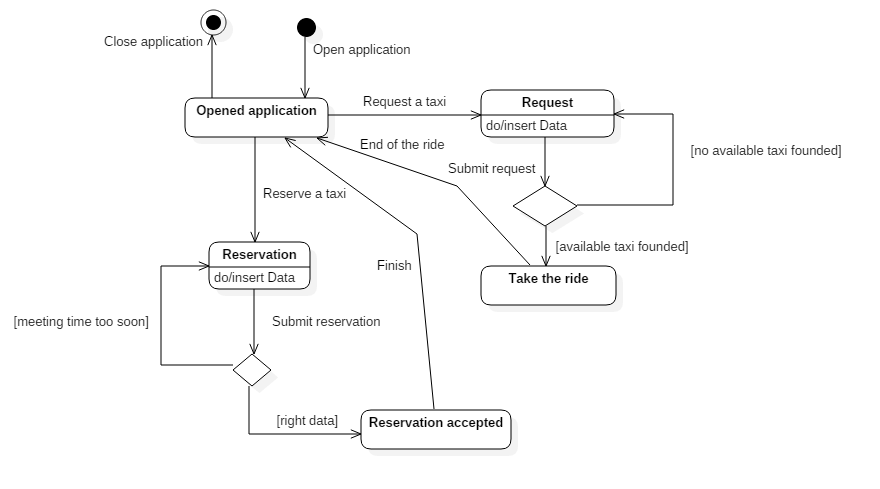
\includegraphics[scale=0.5]{Images/statechart_passenger}
\end{figure}
\subsection{Taxi Driver behavior}
\begin{figure}[H]
\centering
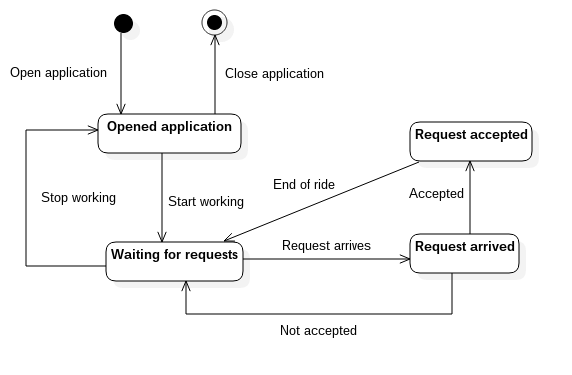
\includegraphics[scale=0.5]{Images/statechart_taxiDriver}
\end{figure}
\section{External interface requirements}
\pagebreak
\section{External interface requirements}
\subsection{User interfaces}
Here we present the mock-ups of the application user interface.\\
We will present the user interface regarding only the two mobile applications (one for the Passengers and one for the Taxi Drivers).\\
The web application interface for the Passenger is a natural extension of the mobile one.
\\
\\
The user interface must be as simple as possible: both the users must be able to use immediately after the installation.
\subsubsection{Home page for the Passenger}
\begin{figure}[H]
\centering
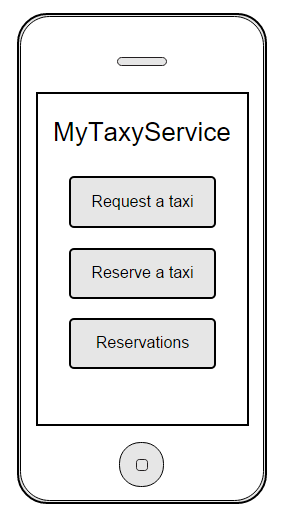
\includegraphics[scale=0.6]{Images/home_page}
\caption{Home page for the Passenger}
\end{figure}
This screen will present to the Passenger the possibility to 
\begin{itemize}
\item Request an immediate taxi service
\item Reserve a taxi for a future journey
\item Check his pending reservations
\end{itemize}

\subsubsection{Request a taxi}
\begin{figure}[H]
\centering
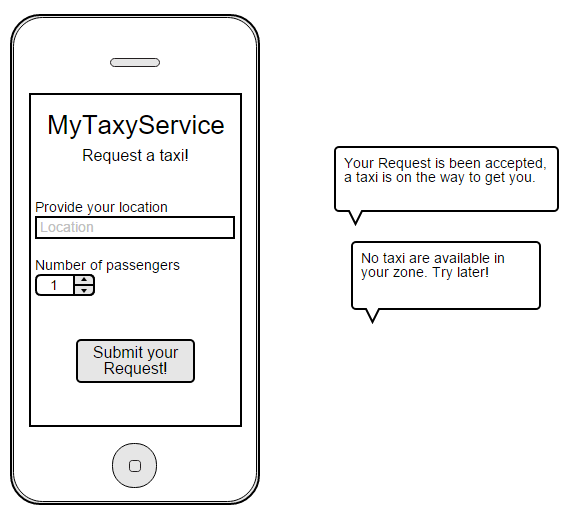
\includegraphics[scale=0.6]{Images/taxi_request}
\caption{Request for an immediate taxi}
\end{figure}
This screen is reached by pressing the button "REQUEST A TAXI" from the Home Page. The user can:
\begin{itemize}
\item Insert his location
\item The number of passengers of the requested ride
\item Submit the request
\end{itemize} 
If one or more necessary information is not inserted (missing) the user will be notified with an appropriate pop-up.


\subsubsection{Reservation of a taxi}
\begin{figure}[H]
\centering
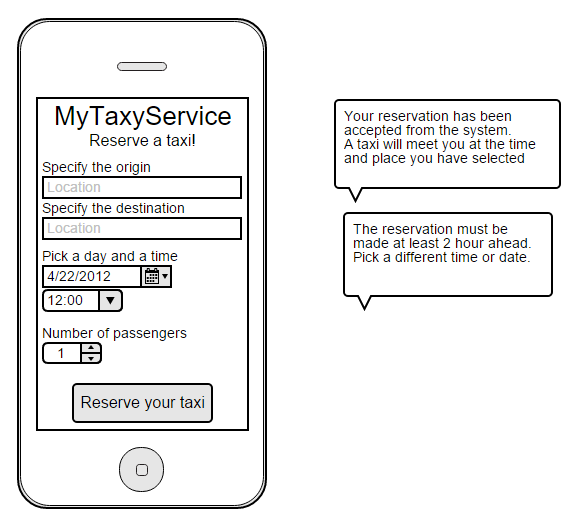
\includegraphics[scale=0.6]{Images/taxi_reservation}
\caption{Reservation of a taxi}
\end{figure}
This screen is reached by pressing the button "RESERVE A TAXI" from the Home Page. The user can:
\begin{itemize}
\item Specify his actual location
\item Specify the destination of the journey
\item Specify the date and hour of the meeting time
\item Specify the number of passengers
\item Submit the reservation request to the system
\end{itemize}
If one or more necessary information is not inserted (missing) the user will be notified with an appropriate pop-up.

\subsubsection{Reservations}
\begin{figure}[H]
	\centering
	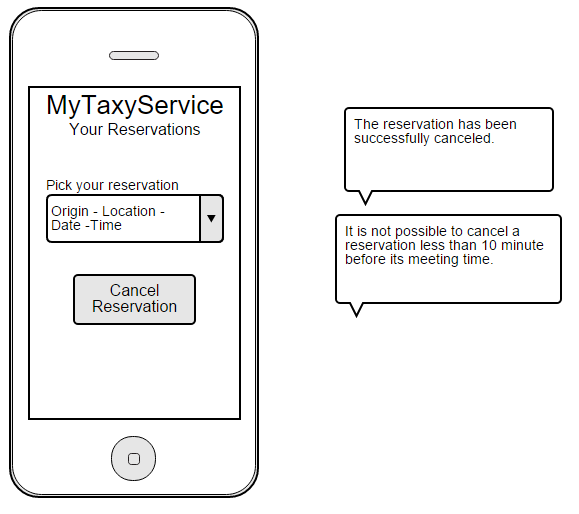
\includegraphics[scale=0.6]{Images/reservations}
	\caption{Reservations page of a passenger}
\end{figure}
This screen is reached by pressing the button "RESERVATIONS" from the Home Page. The user can:
\begin{itemize}
	\item View all the reservations
	\item Cancel a reservation
\end{itemize}
The permission of cancelling a reservation will be granted only if this is done at least 10 minutes before the meeting time. A pop-up will notify the passenger of the result of the operation.

\subsubsection{Acknowledgement of a taxi request/reservation to a Passenger}
\begin{figure}[H]
\centering
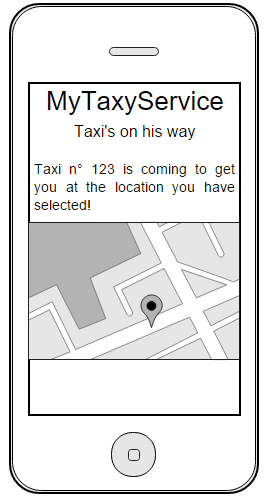
\includegraphics[scale=0.6]{Images/taxi_coming}
\end{figure}
This screen is reached when a taxi is allocated to the Passenger request, both in case of immediate request and reservation.\\
The screen will present:
\begin{itemize}
\item Taxi identification number
\item Waiting time
\item Resume of the submitted data by the Passenger (meeting location, ecc...)
\end{itemize}

\subsubsection{Start working day for a Taxi Driver}
This is the first screen a Taxi Driver will see at the opening of the application:
\begin{figure}[H]
\centering
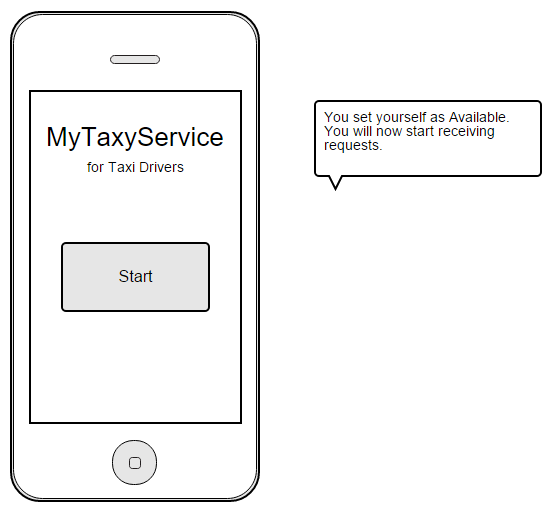
\includegraphics[scale=0.6]{Images/start_taxi_driver}
\caption{First screen of the application for Taxi Drivers}
\end{figure}

\subsubsection{Taxi Driver's waiting for a requests}
\begin{figure}[H]
\centering
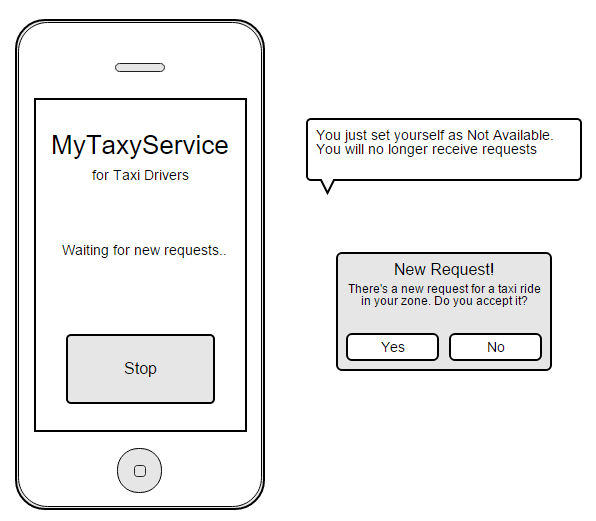
\includegraphics[scale=0.6]{Images/wait_taxi_driver}
\caption{Waiting screen for a taxi driver}
\end{figure}
This screen is reached by pressing on the "START" button on the previous screen.\\
Once a request is submitted to the taxi driver the application notifies him with a pop-up saying that there is a request for a ride in the current zone.\\
It is asked to the taxi driver if he wants to accept the request or not.

\subsubsection{Communication of the location to a Taxi Driver}
\begin{figure}[H]
\centering
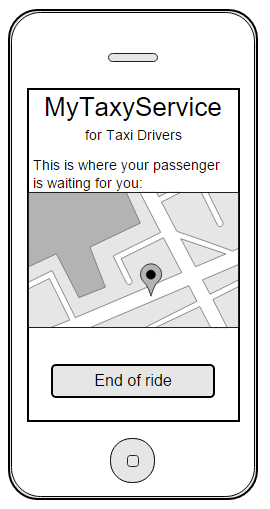
\includegraphics[scale=0.6]{Images/taxi_driver_busy}
\caption{Communication of the Passenger location to the Taxi Driver}
\end{figure}
This screen is reached by pressing the "YES" button on the pop-up displayed on the previous screen. It will be present a map indicating the position of the Passenger (meeting location). When the ride will be done the Taxi Driver will press the "END OF RIDE" button to notify his availability.


\subsection{GUI state chart}
We can summarize the behavior of the user interface through a state chart in which every state represents a specific screen of the application and each transition is basically a user input or a system communication to the application.
\subsubsection{Taxi driver usage of the user interface}
\begin{figure}[H]
\centering
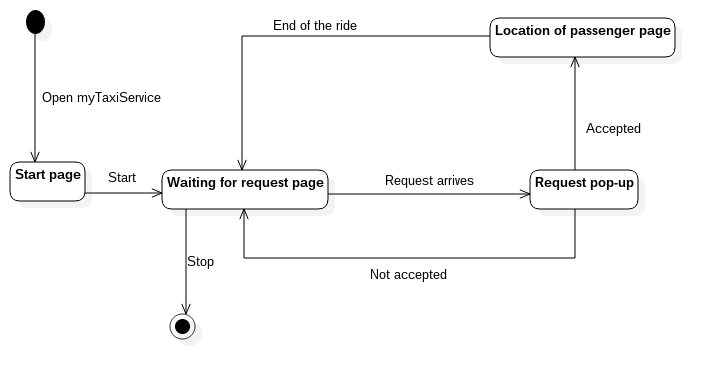
\includegraphics[scale=0.5]{Images/statechart_GUI}
\end{figure}

\subsubsection{Passenger usage of the user interface}
\begin{figure}[H]
\centering
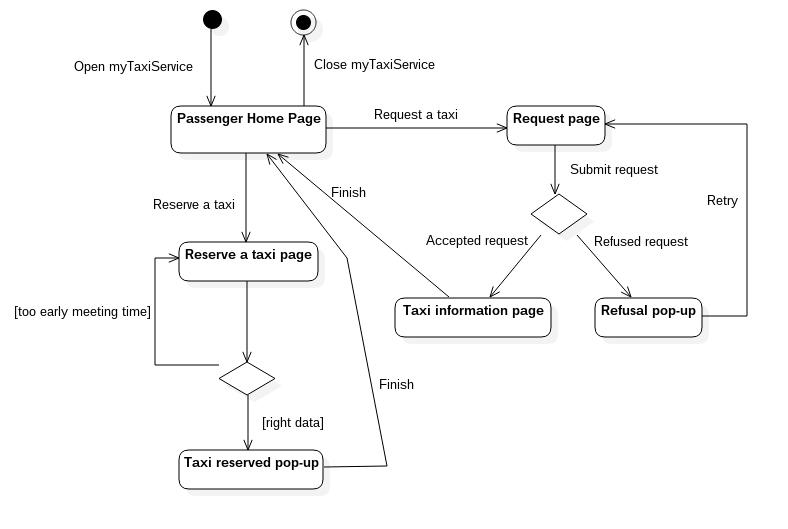
\includegraphics[scale=0.5]{Images/statechart_GUI_Passenger}
\end{figure}
\subsection{Software interfaces}
\subsection{Communication interfaces}
The only communication protocol used is HTTP.

\section{Functional requirements}
\subsection{User class 1}
\subsubsection{Functional requirement 1.1}
\subsection{User class 2}
\subsubsection{Functional requirement 2.1}

\section{Performance requirements}
\section{Design constraints}
\section{Software system attributes}
\section{Other requirements}